\UseRawInputEncoding
\documentclass[12pt]{article}
\usepackage[utf8]{inputenc}
\usepackage{graphicx}
\usepackage{hyperref}
\usepackage[a4paper, total={6in, 8in}]{geometry}
\usepackage[nodisplayskipstretch]{setspace}

\begin{document}

    \pagenumbering{gobble}

    \begin{center}
        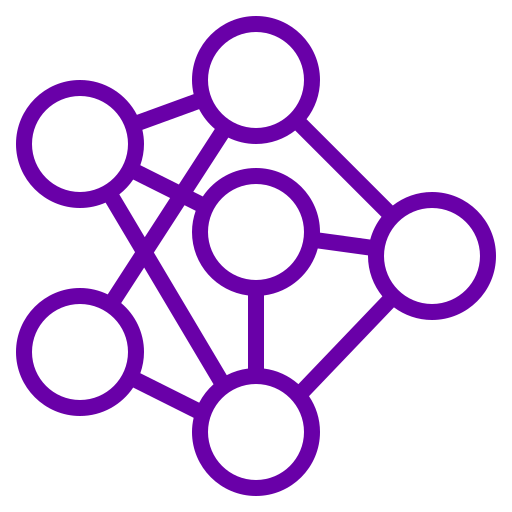
\includegraphics[scale=0.25]{favicon.png} % favicon made by Becris on flaticon.com
        \vspace{15px}

        {\fontfamily{Inconsolata}\selectfont
            \textbf{\LARGE{TUMGAD - Exercises}}\\
         
        }
    \end{center}
    \begin{center}
        \textbf{\LARGE{-----Disclaimer and infos:-----}}
        \\[0.2in]
    \end{center}
    \large{ % rules in place for this specific instance of the game
        1. You can find explanations to all the components in this repository \href{https://sebastianoner.github.io/TUMGAD/src/routes}{\underline{here}}
        \\[0.2in]
        2. This paper was generated by an automated software. It will likely contain flaws. If you find one, please report it
        \href{https://github.com/SebastianOner/TUMGAD/issues/new?assignees=&labels=&template=bug_report.md&title=}{\underline{here}}.
        \\[0.2in]
        3. TUMGADs creators are not affiliated with the lecture organization whatsoever, the exercises/explanations are not
        guaranteed to be accurate or complete.
        \\[0.2in]
        4.
    }
\end{document}